\chapter{Wstęp}

\section{Używany sprzęt oraz narzędzia}

\begin{itemize}
    \item Stanowisko - \textbf{7}
    \item Oscyloskop - \textbf{MSO3012}
    \item Generator funkcyjny - \textbf{AFG3022B}
    \item Płytka RLC - \textbf{05}
    \item Multimetr - \textbf{3}
    \item Wartości eksperymentalne oraz wykresy dla charakterystyk częstotliwościowych zostały sporządzone za pomocą programu \textbf{Origin 2022}
\end{itemize}

\section{Jednostki i przedrostki}

\begin{itemize}
    \item 1 Hz (herc) - jednostka miary częstotliwości - 1Hz = $\frac{1}{1s} = 1s^{-1}$
    \item 1 A (amper) - jednostka natężenia prądu elektrycznego - 1A = $\frac{1C}{1s}$
    \item 1 V (wolt) - jednostka potencjału elektrycznego, napięcia elektrycznego i siły elektromotorycznej - 1V = $\frac{1W}{1A}$ ($\frac{wat}{amper}$)
    \item 1 F (farad) - jednostka pojemności elektrycznej - 1F = $\frac{1C}{1V}$ ($\frac{kulomb}{wolt}$)
    \item 1 H (henr) - jednostka indukcyjności - 1H = $\frac{1 Wb}{1 A}$ ($\frac{weber}{amper})$
\end{itemize}

\begin{itemize}
    \item k (kilo) = $10^3$
    \item m (mili) = $10^{-3}$
    \item \micro (micro) = $10^{-6}$
    \item n (nano) = $10^{-9}$
\end{itemize}

\section{Funkcja przejścia T($\omega$)}

Sprzężenie wyjścia z wejściem. T = $\dfrac{odpowiedz}{wymuszenie}.$ \\

\begin{equation}
T(\omega) = \frac{Z_2(\omega)}{Z_1(\omega)+Z_2(\omega)}
\end{equation}
$Z_1/Z_2$ - impedancja

\section{Stała czasowa $\tau$}

\begin{center} $\tau$ = R $\cdot$ C \end{center}
R - rezystancja rezystora \\
C - pojemność kondensatora \\

\section{Czwórnik RC}

Czwórnik RC to:
\begin{itemize}
    \item filtr dolnoprzepustowy
    \item układ całkujący
\end{itemize}

Schemat czwórnika:

\begin{figure}[H]
    \centering
    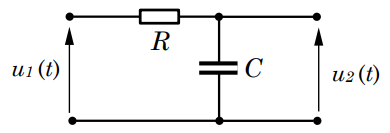
\includegraphics[scale=0.75]{img_wyklad/RC.png}
    \caption{Czwórnik RC}
    \label{fig:RC}
\end{figure}

\section{Czwórnik CR}


Czwórnik CR to: 
\begin{itemize}
    \item filtr górnoprzepustowy
    \item układ różniczkujący
\end{itemize}

Schemat czwórnika:

\begin{figure}[H]
    \centering
    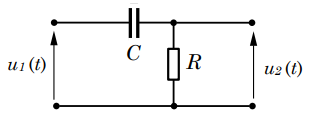
\includegraphics[]{img_wyklad/CR.png}
    \caption{Czwórnik CR}
    \label{fig:CR}
\end{figure}

\section{Czwórnik CLR}

Schemat czwórnika:

\begin{figure}[H]
    \centering
    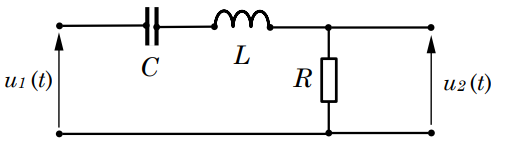
\includegraphics[scale=0.6]{img_wyklad/CLR.png}
    \caption{Czwórnik CLR}
    \label{fig:CLR}
\end{figure}

\section{Charakterystyka amplitudowa}
\label{poprawa:charakterystyka_amplitudowa}

Funkcja określająca zależność $|T|$ od częstości. \\
Charakterystyka amplitudowa dla czwórników CR i RC:
\begin{figure}[H]
    \centering
    \begin{subfigure}[h]{0.45\textwidth}
        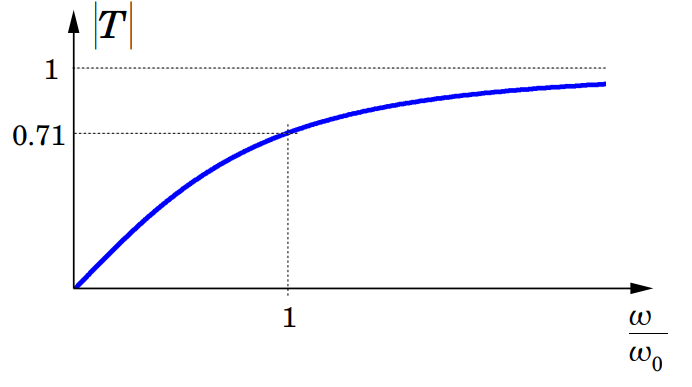
\includegraphics[width=\textwidth]{img_wyklad/teor_amp_CR.png}
        \caption*{Charakterystyka amplitudowa czwórnika CR}
    \end{subfigure}
    \begin{subfigure}[h]{0.45\textwidth}
        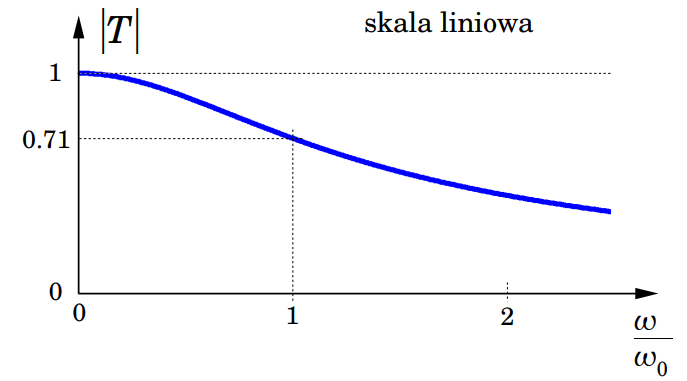
\includegraphics[width=\textwidth]{img_wyklad/teor_amp_RC.png}
        \caption*{Charakterystyka amplitudowa czwórnika RC}
    \end{subfigure}
\end{figure}

\section{Charakterystyka fazowa}
\label{poprawa:charakterystyka_fazowa}

Funkcję określającą zależność $\phi$ od częstości nazywamy charakterystyką fazową. \\
Charakterystyka fazowa dla czwórników CR i RC:
\begin{figure}[H]
    \centering
    \begin{subfigure}[h]{0.45\textwidth}
        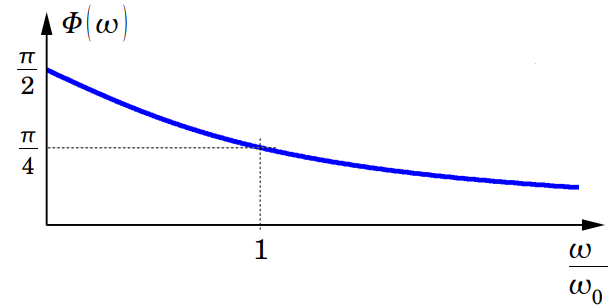
\includegraphics[width=\textwidth]{img_wyklad/teor_faza_CR.png}
        \caption*{Charakterystyka fazowa czwórnika CR}
    \end{subfigure}
    \begin{subfigure}[h]{0.45\textwidth}
        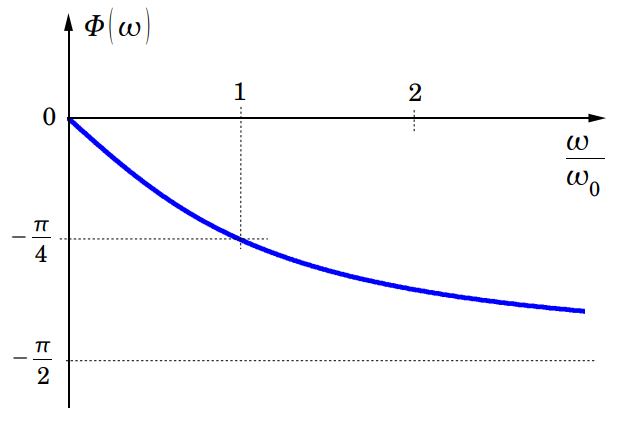
\includegraphics[width=\textwidth]{img_wyklad/teor_faza_RC.png}
        \caption*{Charakterystyka fazowa czwórnika RC}
    \end{subfigure}
\end{figure}